%%%%%%%%%%%%%%%%%%%%%%%%%%%%%%%%%%%%%%%%%%%%%%%%%%%%%%
% A Beamer template for University of Wollongong     %
% Based on THU beamer theme                          %
% Author: Qiuyu Lu                                   %
% Date: July 2024                                    %
% LPPL Licensed.                                     %
%%%%%%%%%%%%%%%%%%%%%%%%%%%%%%%%%%%%%%%%%%%%%%%%%%%%%%
% Customized for Sharif University of Technology     %
%%%%%%%%%%%%%%%%%%%%%%%%%%%%%%%%%%%%%%%%%%%%%%%%%%%%%%


\documentclass[serif, aspectratio=169]{beamer}
%\documentclass[serif]{beamer}  % for 4:3 ratio
\usepackage[T1]{fontenc} 
\usepackage{fourier} % see "http://faq.ktug.org/wiki/uploads/MathFonts.pdf" for other options
\usepackage{hyperref}
\usepackage{latexsym,amsmath,xcolor,multicol,booktabs,calligra}
\usepackage{graphicx,pstricks,listings,stackengine}
\usepackage{lipsum}
\usepackage{tikz}
% For writing clean pseudocodes
% \usepackage{algorithm, algpseudocode, mathtools, needspace}
% \usepackage{algorithmic}
\usepackage{algorithm}
\usepackage{algorithmic}
\usepackage{algpseudocode}

% To justify the items


\author{Ali Sharifi-Zarchi}
% \author{CE Department}
\title{Machine Learning (CE 40477)}
\subtitle{Fall 2024}
\institute{
    CE Department \\
    Sharif University of Technology
}
%\date{\small \today}
% \usepackage{UoWstyle}
\usepackage{SUTstyle}

% defs
\def\cmd#1{\texttt{\color{red}\footnotesize $\backslash$#1}}
\def\env#1{\texttt{\color{blue}\footnotesize #1}}
\definecolor{deepblue}{rgb}{0,0,0.5}
\definecolor{deepred}{RGB}{153,0,0}
\definecolor{deepgreen}{rgb}{0,0.5,0}
\definecolor{halfgray}{gray}{0.55}

\lstset{
    basicstyle=\ttfamily\small,
    keywordstyle=\bfseries\color{deepblue},
    emphstyle=\ttfamily\color{deepred},    % Custom highlighting style
    stringstyle=\color{deepgreen},
    numbers=left,
    numberstyle=\small\color{halfgray},
    rulesepcolor=\color{red!20!green!20!blue!20},
    frame=shadowbox,
}

% For writing comments that are aligned to the left side
\makeatletter
\NewDocumentCommand{\LeftComment}{s m}{%
  \Statex \IfBooleanF{#1}{\hspace*{\ALG@thistlm}}\(\triangleright\) #2}
\makeatother
% To manually indent states in algorithmicx
\newcommand{\IndState}{\State\hspace{\algorithmicindent}}
% To make breakable algorithms
\makeatletter
\newenvironment{nofloatalgorithmic}[2][0]
  {
  \par
  \needspace{\dimexpr\baselineskip+6.8pt}
  \noindent
  \hrule height.8pt depth0pt \kern2pt
  \refstepcounter{algorithm}
  \addcontentsline{loa}{algorithm}{\numberline{\thealgorithm}#2}
  \noindent\textbf{\fname@algorithm~\thealgorithm} #2\par
  \kern2pt\hrule\kern2pt
  \begin{algorithmic}[#1]
  }
  {
  \end{algorithmic}
  \nobreak\kern2pt\hrule\relax
  }
\makeatother
% To make vertical arrow
\newcommand\vertarrowbox[3][6ex]{%
  \begin{array}[t]{@{}c@{}} #2 \\
  \left\uparrow\vcenter{\hrule height #1}\right.\kern-\nulldelimiterspace\\
  \makebox[0pt]{\scriptsize#3}
  \end{array}%
}
% Clean argmin
\DeclareMathOperator*{\argmin}{arg\,min}


\begin{document}

\begin{frame}
    \titlepage
    \vspace*{-0.6cm}
    \begin{figure}[htpb]
        \begin{center}
            
\includegraphics[keepaspectratio, scale=0.25]{pic/sharif-main-logo.png}
        \end{center}
    \end{figure}
\end{frame}

\begin{frame}    
\tableofcontents[sectionstyle=show,
subsectionstyle=show/shaded/hide,
subsubsectionstyle=show/shaded/hide]
\end{frame}

\section{Unsupervised Learning Overview}
\begin{frame}{Unsupervised Learning}
    \textbf{Unsupervised Learning} involves working with \textbf{unlabeled data}, where the goal is to \textbf{infer the natural structure} present within a set of data points.
    \begin{itemize}
        \item Learning from unlabeled data.
        % \item Most of the times, there is no (or minimal) prior knowledge of the data.
        \item Two of the most common tasks:
        \begin{itemize}
            \item \textbf{Clustering}: Grouping data points into clusters based on similarity towards user need.
            \item \textbf{Dimensionality Reduction}: Reducing the number of features under consideration and keeping (perhaps approximately) the most informative features.
        \end{itemize}
    \end{itemize}
\end{frame}

\begin{frame}{Music Recommendation Systems }
\begin{itemize}
    \item When you like a song you probably like other "similar" songs.
    \item Fun little exercise to \href{https://machinelearninggeek.com/spotify-song-recommender-system-in-python/}{build a simple system}, after finishing this chapter.
\end{itemize}
  
    \begin{figure}
        \centering
        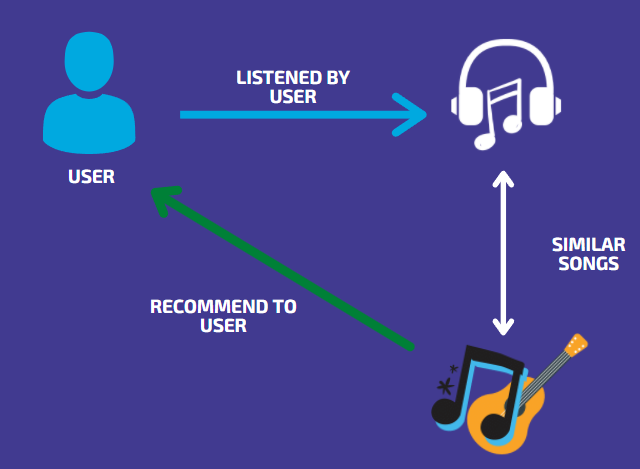
\includegraphics[scale=0.3]{pic/figs/image-4.png}
    \end{figure}
    
    \begin{tikzpicture}[Simple Music Recommendation]
        \node[anchor=south west, xshift=0.1cm, yshift=0.22cm] at (current page.south west) {
            \scriptsize Figure adapted from \href{https://machinelearninggeek.com/spotify-song-recommender-system-in-python/}{machinelearninggeek.com}
        };
    \end{tikzpicture}

\end{frame}


\begin{frame}{Music Recommendation Systems }
\begin{itemize}
    \item When you like a song you probably like other "similar" songs.
    \item Fun little exercise to \href{https://machinelearninggeek.com/spotify-song-recommender-system-in-python/}{build a simple system}, after finishing this chapter.
\end{itemize}

    \begin{figure}
        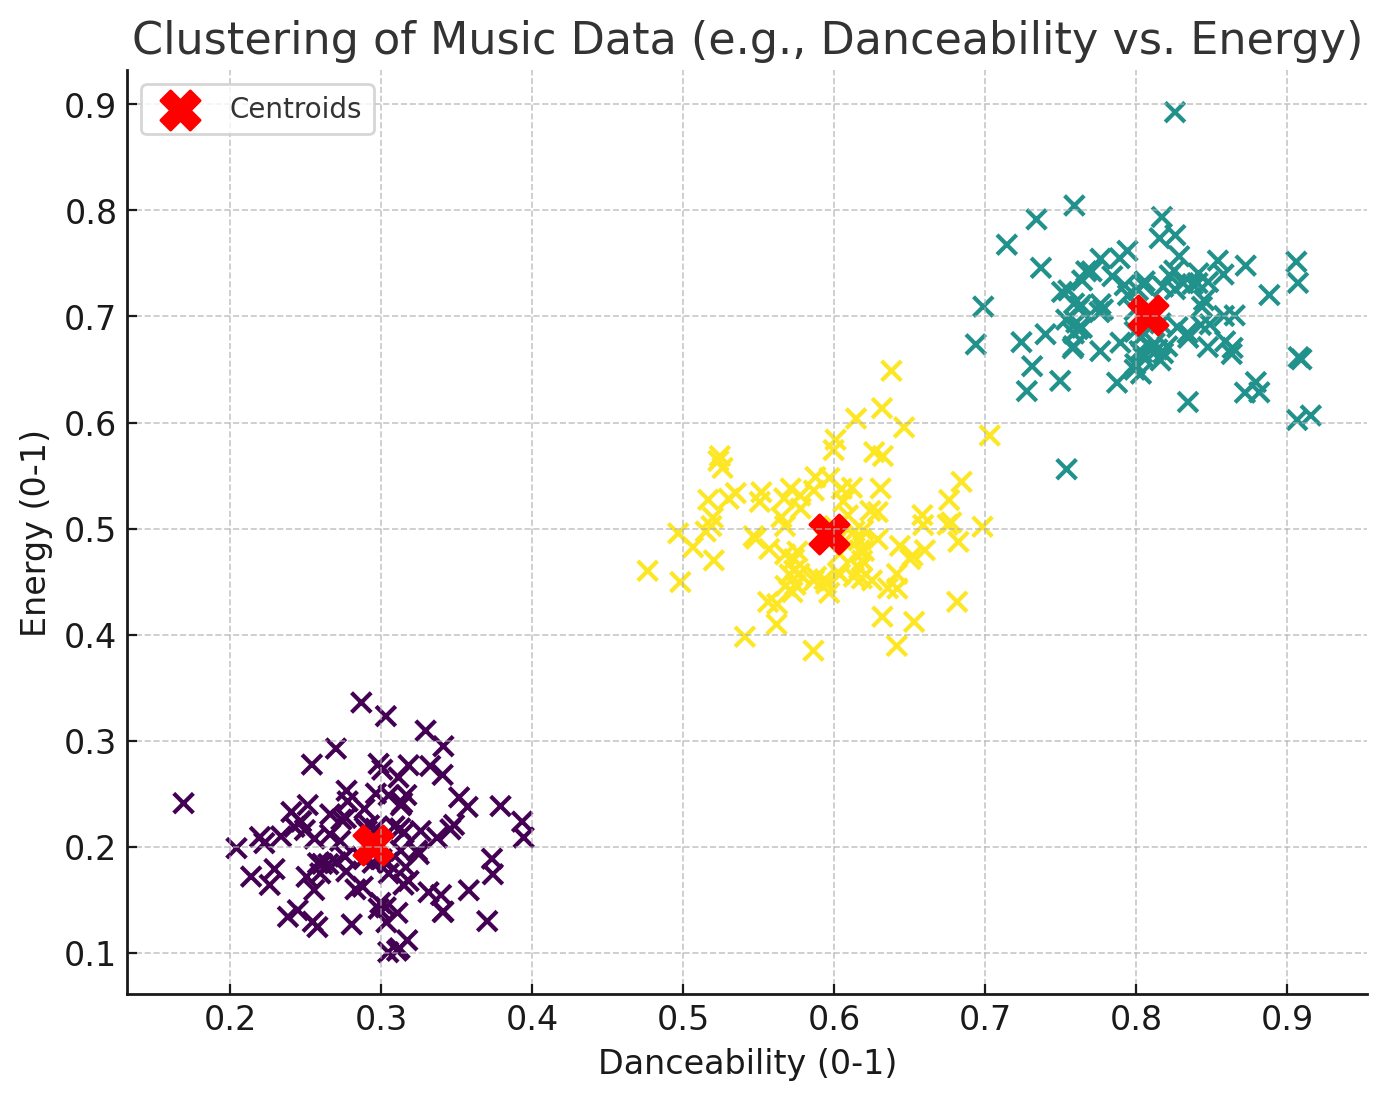
\includegraphics[scale=0.4]{pic/figs/Music Clustering2.png}
        \centering
    \end{figure}

        
\end{frame}

\begin{frame}{Organizing Photos on Smartphones }
\begin{itemize}
    \item All pictures with that one friend
    \item All pictures where you looked "cool"
\end{itemize}
    \begin{figure}
        \centering
        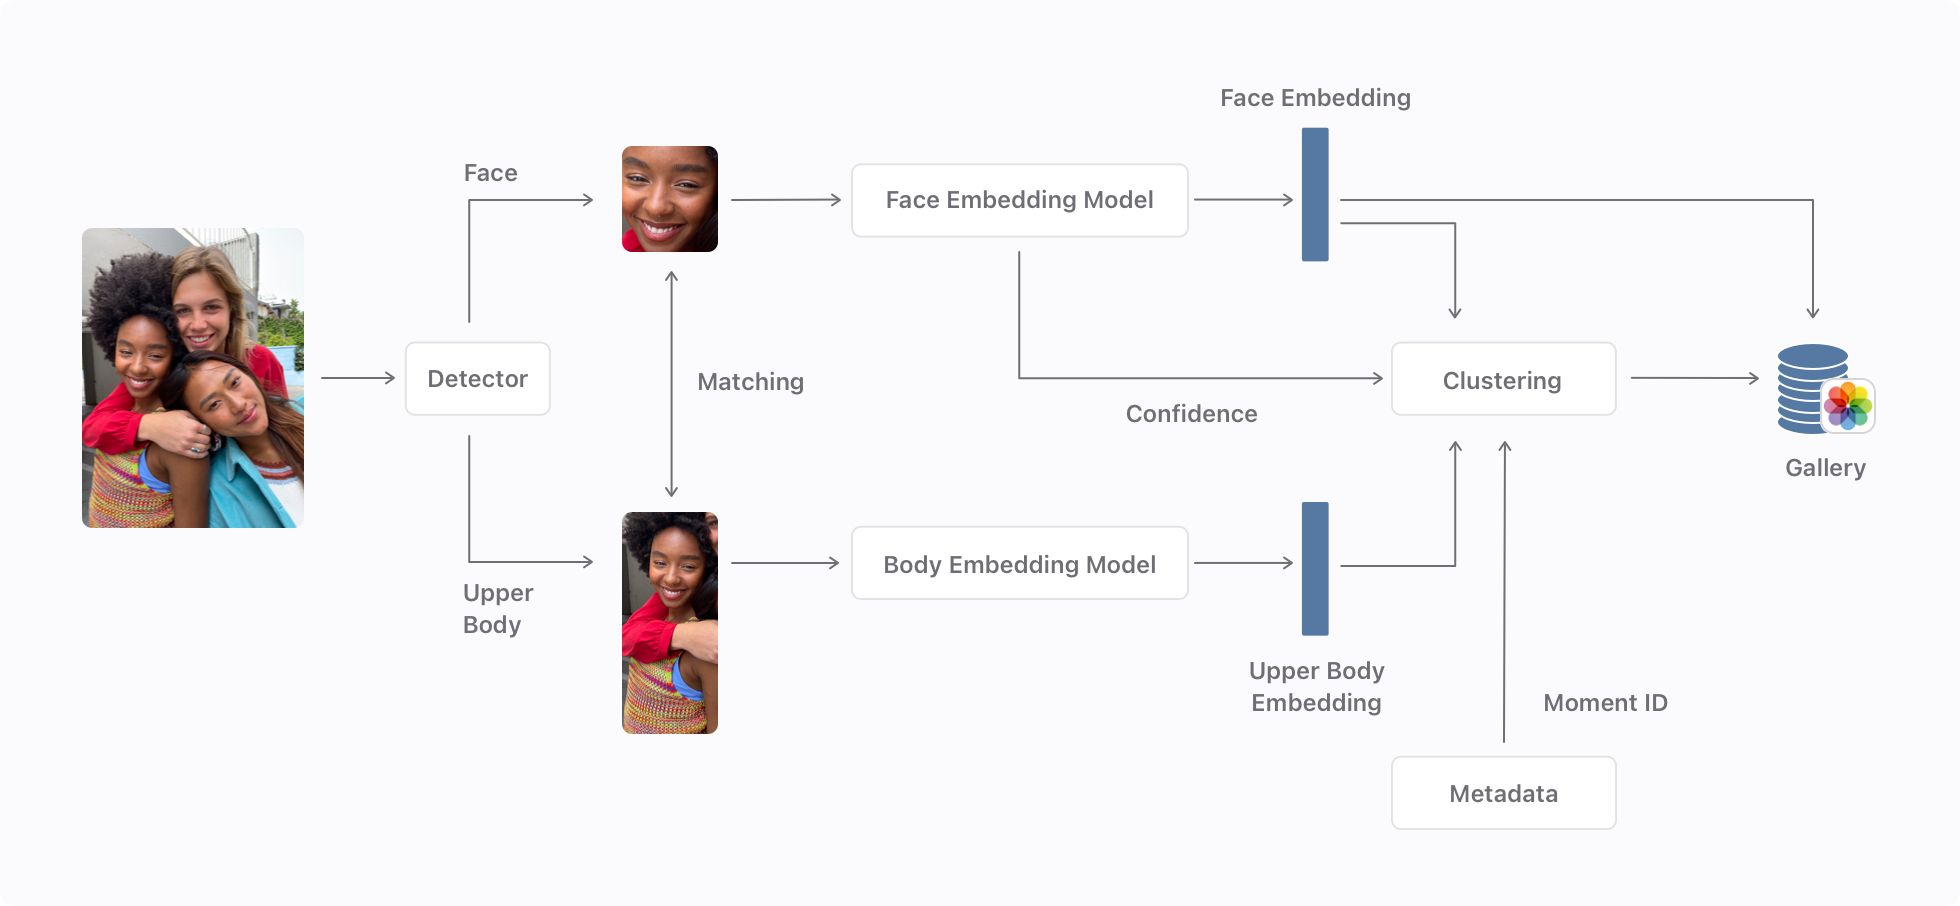
\includegraphics[scale=0.2]{pic/figs/rec_people_fig2_3f04b0c03f.jpg}
    \end{figure}
    
    
    \begin{tikzpicture}[Recognizing people in image collections]
        \node[anchor=south west, xshift=0.1cm, yshift=0.22cm] at (current page.south west) {
            \scriptsize Recognizing people in image collections. Figure from \href{https://machinelearning.apple.com/research/recognizing-people-photos}{Apple Research}. 
        };
    \end{tikzpicture}
\end{frame}

\section{K-Means}
\begin{frame}{K-Means overview}
    \begin{itemize}
        \item   A popular \textbf{clustering} algorithm
        \item \textbf{Similar} data in the same cluster.
        \item K-Means suggests an \textbf{iterative} process to find these centers.
        \begin{figure}
        \centering
        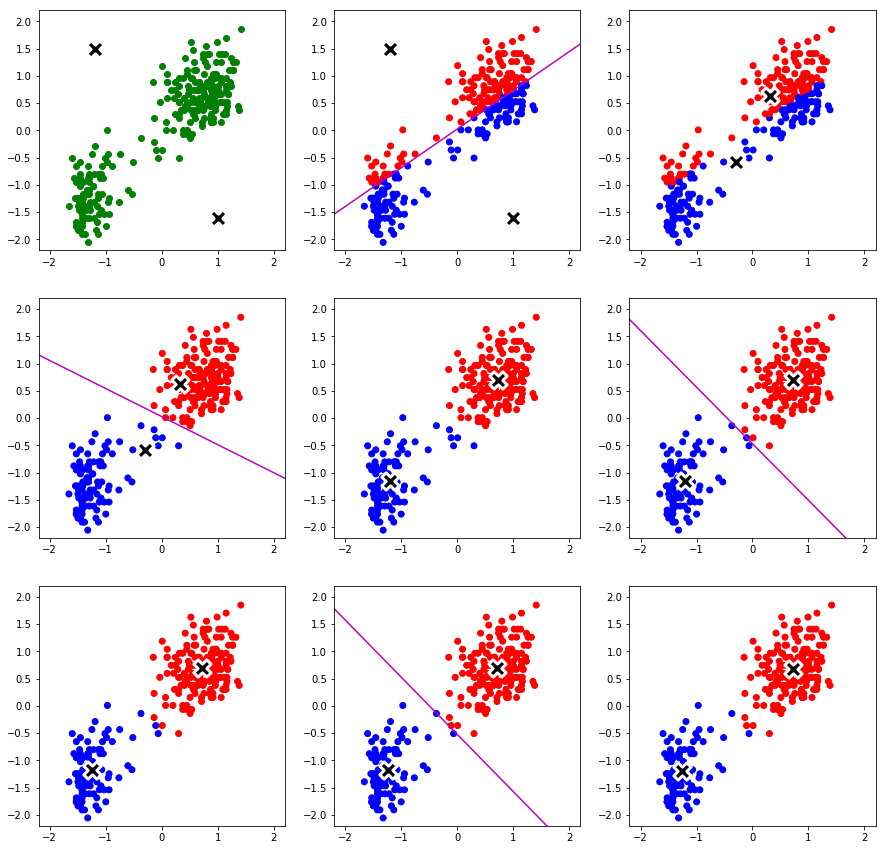
\includegraphics[scale=0.18]{pic/figs/Clustering_K-means_7_1.png}
        Figure From \href{https://mlbhanuyerra.github.io/2018-02-19-Clustering-K-means/}{mlbhanuyerra.github.io}.
    \end{figure}
    \end{itemize}
\end{frame}

\begin{frame}{Problem Intuition}
    \begin{itemize}
    
        \item One of the most straightforward tasks we can perform on a data set without labels.
        \item finding groups of data in our dataset which are "similar" to one another --\textbf{clusters}.
        \item How many cluster? Can we cluster new unseen data? What is similar data ?
    \end{itemize}
\end{frame}


\begin{frame}{Problem definition}
    \begin{itemize}
        \item Formally: We have $X_{\text{train}} = \{ x^{(1)}, x^{(2)}, \dots, x^{(N)} \} \subseteq \mathbb{R}^d$
        \item Assume we know there are $K$ clusters, or we want $K$ clusters.
        \item We are learning:
        \begin{enumerate}
            \item a function or mapping $f:\mathbb{R}^d\to \{1,2, \dots , K\}$ that assigns a cluster to each data point.
            \item a set of \( K \) prototypes \(\mu = \{ \mu_1, \mu_2, \dots, \mu_K  \} \subseteq \mathbb{R}^d \) as the \textbf{cluster representatives}.
        \end{enumerate}
        \item data assigned to the same $i \in \{1,2, \dots , K\}$ are in the same cluster $i$.
    \end{itemize}
\end{frame}

\begin{frame}{Objective Function}
\begin{itemize}
    
    \item Create objective function like the loss we had before.
    \item We want data in the same cluster to be closer and data from different clusters to be further. more on this later.
    \item in K-Means, this is expressed as:

    $$
    \sum_{\mathbf{x} \in X_{\text{train}}} || x -  \mu_{f(x)} ||^2
    $$
    
\end{itemize}
\end{frame}


\begin{frame}{Objective Function (cont.)}
    \begin{itemize}
        
        \item We can express $f$ by defining $r_k(\mathbf{x}) = 1$ if $f(\mathbf{x}) = k$ and $0$ otherwise, we can write this objective as below:
$$
J = \sum_{\mathbf{x} \in X_{\text{train}}} \sum_{k=1}^{K} r_k(x)|| x -  \mu_k ||^2
$$
        \item called\textit{distortion measure}.
        \item chose $f$ and $\mu$ to minimize this.
        \item Its NP-hard. what does K-Means suggest ?
      
    \end{itemize}
\end{frame}

\begin{frame}{Observation}
    \begin{itemize}

\item If we fix the set of \textbf{centroids} or representatives $\mu$, we could minimize each term by \textbf{assigning}:
  $$ f(x) : = \textit{argmin}_k \; ||x - \mu_k||^2 $$.
  
    \end{itemize}
\end{frame}

\begin{frame}{Observation (cont.)}
    
     If we fix the assignments $f$ we can optimize for $\mu$ by taking the derivative as:
    $$
        \frac{\partial J}{\partial \mu_k } = 0 \implies 2 \sum_{i=1}^{N} r_k(x_i) \left(x_i - \mu_k \right) = 0
    $$
and \textbf{updating} $\mu$ as:
    $$
        \mu_k = \frac{\sum_{i=1}^{N}{r_k(x_i)x_i}}{\sum_{i=1}^{N} r_k(x_i)}
    $$

\end{frame}

\begin{frame}{K-Means Process}
\begin{itemize}
\item K-Means uses an iterative process that:
\begin{enumerate}
    \item \textbf{Assigns} each point to the \textbf{nearest} centroid. Optimizing for $f$.
    \item \textbf{Updates} each centroid as the \textbf{mean} of the points in its cluster. Optimizing for $\mu$.
\end{enumerate}

% \begin{figure}
%     \centering
%     \includegraphics[width=0.5\linewidth]{}
%     \caption{Caption}
%     \label{fig:enter-label}
% \end{figure}

    \end{itemize}
\end{frame}

% K means in action
\begin{frame}{K-Means in action}
original blobs
    \begin{figure}
        \centering
        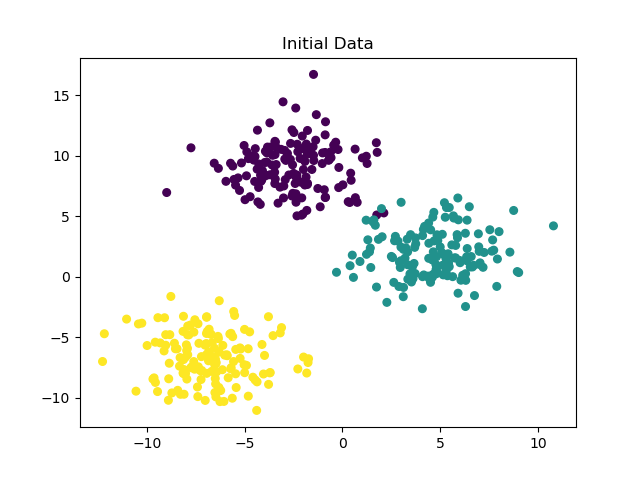
\includegraphics[scale=0.45]{kmeans_in_action_figures/original.png}
    \end{figure}
\end{frame}

\begin{frame}{K-Means in action}
random initialization
    \begin{figure}
        \centering
        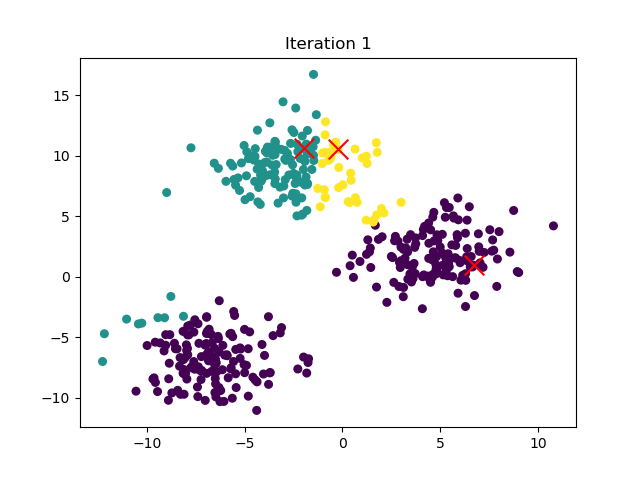
\includegraphics[scale=0.45]{kmeans_in_action_figures/kmeans_iter_1.png}
    \end{figure}
\end{frame}
\begin{frame}{K-Means in action (cont.)}
    \begin{figure}
        \centering
        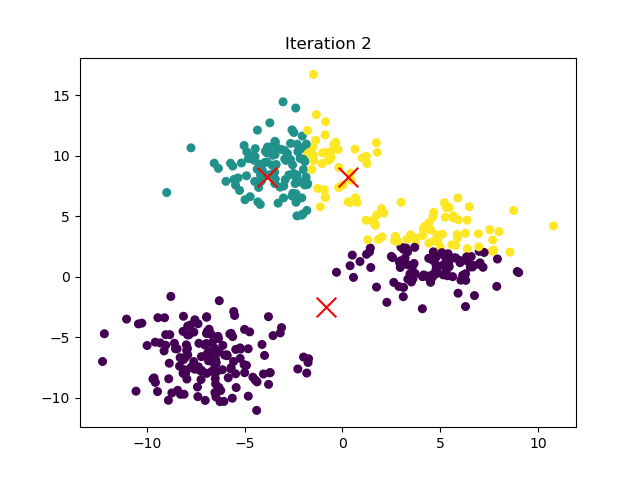
\includegraphics[scale=0.45]{kmeans_in_action_figures/kmeans_iter_2.png}
    \end{figure}
\end{frame}

\begin{frame}{K-Means in action (cont.)}
    \begin{figure}
        \centering
        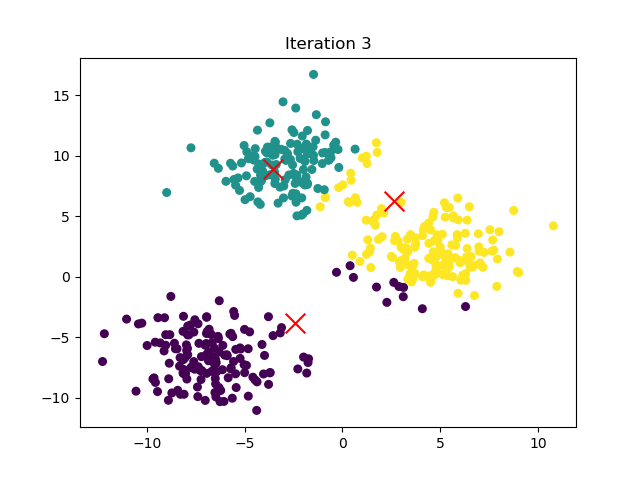
\includegraphics[scale=0.45]{kmeans_in_action_figures/kmeans_iter_3.png}
    \end{figure}
\end{frame}
\begin{frame}{K-Means in action (cont.)}
    \begin{figure}
        \centering
        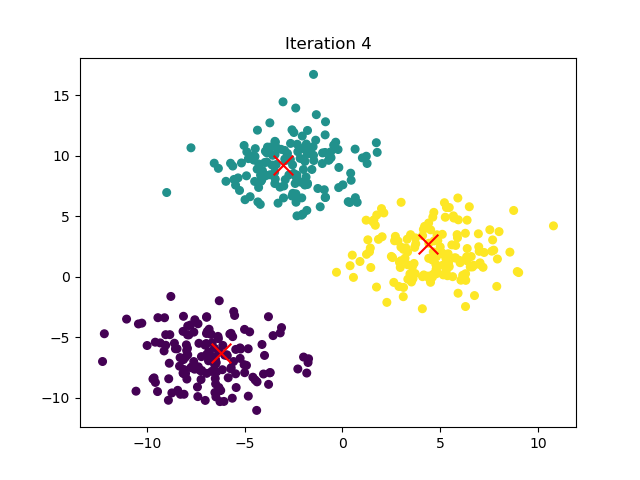
\includegraphics[scale=0.45]{kmeans_in_action_figures/kmeans_iter_4.png}
    \end{figure}
\end{frame}
\begin{frame}{K-Means in action (cont.)}
    \begin{figure}
        \centering
        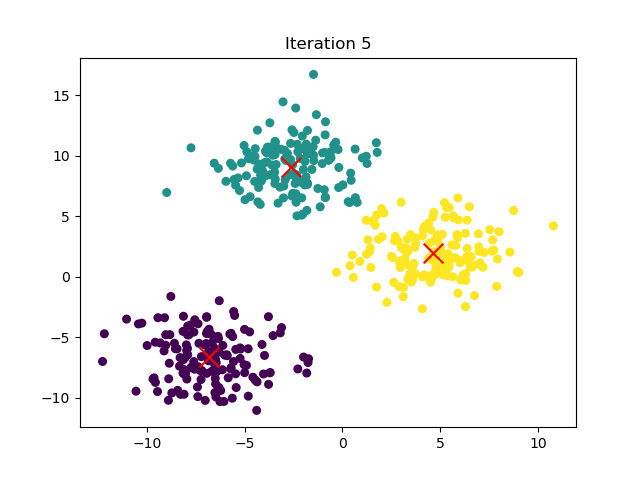
\includegraphics[scale=0.45]{kmeans_in_action_figures/kmeans_iter_5.png}
    \end{figure}
\end{frame}


\begin{frame}{K-Means Algorithm}
 \resizebox{\textwidth}{!}{%
\begin{algorithm}
\caption{K-means Clustering Algorithm}
\begin{algorithmic}[1]
\State \textbf{Input:} Data points $X = \{x_1, x_2, ..., x_n\} \subset \mathbb{R}^d$, number of clusters $K$
\State \textbf{Output:} Clusters $C = \{C_1, C_2, ..., C_K\}$ and centroids $\mu = \{\mu_1, \mu_2, ..., \mu_K\}$
\State \textbf{Initialize:} Randomly select $K$ points as initial centroids $\mu_1, \mu_2, ..., \mu_K$
\end{algorithmic}
\end{algorithm}
}
\end{frame}


\begin{frame}{K-Means Algorithm (cont.)}
 \resizebox{\textwidth}{!}{%
\begin{algorithm}
\caption{K-means Clustering Algorithm (cont.)}
\begin{algorithmic}[2]
\Repeat
    \State \textbf{Assignment step:}
    \For {each data point $x_i$}
        \State Assign $x_i$ to the nearest cluster $C_k$: 
        \[
        C_k = \{ x_i : ||x_i - \mu_k||^2 \leq ||x_i - \mu_j||^2, \, \forall j = 1, 2, ..., K \}
        \]
    \EndFor
    \State \textbf{Update step:}
    \For {each cluster $C_k$}
        \State Update the centroid of $C_k$: 
        \[
        \mu_k = \frac{1}{|C_k|} \sum_{x_i \in C_k} x_i
        \]
    \EndFor
\Until{the centroids do not change (convergence)}
\end{algorithmic}
\end{algorithm}
}
\end{frame}

\begin{frame}{Algorithm Overview}
    \begin{figure}
        \centering
        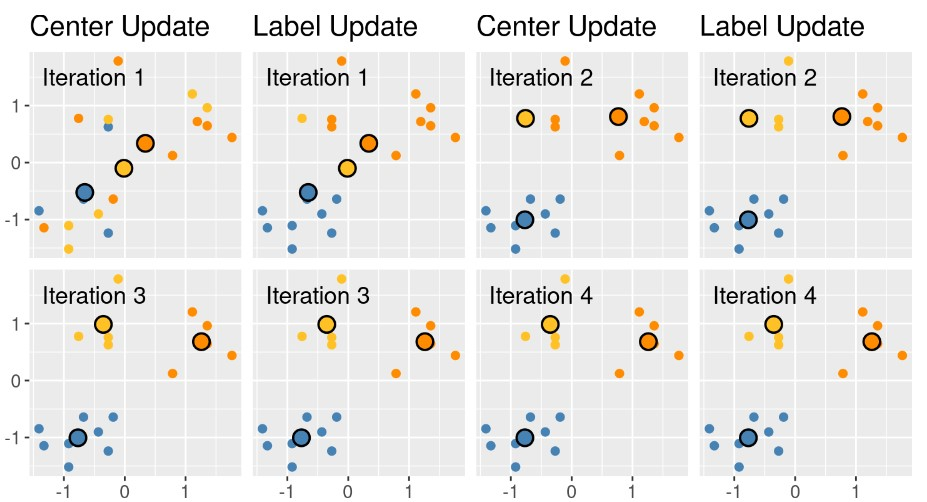
\includegraphics[scale=0.45]{pic/figs/actionmeans.jpg}
        \caption{picture from \href{https://datasciencebook.ca/clustering.html}{datasciencebook.ca}}
    \end{figure}
\end{frame}

\begin{frame}{Convergence}
    \begin{itemize}
    \item How do we know K-Means will converge in a finite number of steps ?
        
    \end{itemize}
\end{frame}

\begin{frame}{Convergence (cont.)}
\begin{itemize}
    \item  In Assignment step:
        \begin{itemize}
        \item  we optimize \( J \) with respect to \( r_k(x) \).
        \item In this step \( J \) is a linear combination of \( r_k(x) \).
        \item We need each $x$ to be at least in some cluster and terms involving different $x$s are independent.
        \item So for each $x$ we chose one of the the $K$ distance expressions that is the minimum. i.e. 
            $$
            r_k(x) = 
            \begin{cases}
                1 & k = \text{argmin}_j ||x-\mu_j ||_2^2 \\
                0 & O.W
            \end{cases}
            $$
            \item This will definitely not decrease $J$.
        \end{itemize}
            
\end{itemize}
    
\end{frame}

\begin{frame}{Convergence (cont.)}
\begin{itemize}
    \item  Now with $r_k$s fixed, $J$ is a quadratic function of $\mu_k$ (like SSE) and by taking derivative we can minimize as:
$$
        \frac{ \partial J }{ \partial \mu_k } = 0 \implies 2 \sum_{i=1}^{N} r_k(x_i) \left(x_i - \mu_k \right) = 0
$$
then we set:
$$
        \mu_k = \frac{\sum_{i=1}^{N}{r_k(x_i)x_i}}{\sum_{i=1}^{N} r_k(x_i)}
$$
\item This will also definitley not increase $J$.

\end{itemize}
    
\end{frame}

\begin{frame}{Convergence (cont.)}
    \begin{itemize}
\item We know each step will not increase the $J$ objective from its current value.
\item  Also and $J$ is non-negative, and there are a finite number of partitions so there is a minimum.
 \item  Therefore we must converge at some point, where the $J$ does not decrease anymore.
\item  The convergence properties of the K-means algorithm were studied by MacQueen (1967).

    \end{itemize}
\end{frame}


\begin{frame}{K-Means convergence (cont.)}
    \begin{figure}
        \centering
        \includegraphics[scale=0.45]{pic/figs/distortion.png}
    \end{figure}
\end{frame}

\begin{frame}{Optional Adventure}
    \item  Each Assignment and Updating step in K-Means corresponds respectively to the E (expectation) and M (maximization) steps of the EM algorithm.
    \item One can prove that k-means is equivalent to running EM on a particular Naive Bayes Model.  
\end{frame}

\begin{frame}{Strengths}
    \begin{itemize}
        \item Simple: easy to understand and to implement.
        \item  Efficient: Time complexity: $O(tkn)$, 
where
\begin{itemize}
    
\item  $n$ is the number of data points, 
\item $k$ is the number of clusters, and 
\item $t$ is the number of iterations. 
\end{itemize}
% – Since both k and t are usually small. k-means is considered a linear algorithm. (personally not sure about this ???)
        
    \end{itemize}
\end{frame}

\begin{frame}{Some Issues}
    \begin{itemize}
        \item k-Means always converges. What could go wrong ?
        \item K-means algorithm is a \textbf{heuristic}
        \item It requires initial centroids, and the choice is important. It could affect the $t$ in $O(tkn)$.
        
        
        
    \end{itemize}
\end{frame}


\begin{frame}{Local optimum}
    \begin{itemize}
        \item The algorithm finds a local Minimum but it does not guarantee global minimum.
        \item This is highly affected by the initialization.
        \item Whats the solution ? some suggestions are:
        \begin{itemize}
            \item variance-based split / merge
            \item Random centers from the data points with Multiple runs and select the best ones.
            \item initialization heuristics (k-means++ , Furthest Traversal)
            \item Initializing with the suggested results of another method
        \end{itemize}
    \end{itemize}
\end{frame}

\begin{frame}{Local optimum}
    \begin{itemize}
        \begin{figure}
            \centering
            \includegraphics[scale=0.55]{pic/original_data.png}
        \end{figure}
    \end{itemize}
\end{frame}
\begin{frame}{Local optimum (cont.)}
    \begin{minipage}{0.5\textwidth}
        \begin{figure}
            \centering
            \includegraphics[scale=0.55]{pic/optimal_clustering.png}
        \end{figure}
        \vfill
        \begin{center}
            Optimal clustering
        \end{center}
    \end{minipage}%
    \begin{minipage}{0.5\textwidth}
        \begin{figure}
            \centering
            \includegraphics[scale=0.55]{pic/possible_clustering.png}
        \end{figure}
        \vfill
        \begin{center}
            Possible clustering
        \end{center}
    \end{minipage}
\end{frame}


\begin{frame}{Defined Mean}
    \begin{itemize}
        \item In the begging we assumed $x_i \in \mathbb{R}^d$, which is not always the case. K-Means requires a space where sample \textbf{mean} is defined.
        \begin{itemize}
            \item A simple case is when we have categorical data. 
            \item  A suggested solution: k-mode - the centroid is represented by most frequent values.
        \end{itemize}


    \end{itemize}
\end{frame}

\begin{frame}{How many clusters?}
    \begin{figure}
        \centering
        \includegraphics[scale=0.5]{pic/how_many_clusters.png}
    \end{figure}
    \begin{tikzpicture}[remember picture,overlay]
        \node[anchor=south west, xshift=0.1cm, yshift=0.22cm] at (current page.south west) {
            \scriptsize Figure adapted from slides of Dr. Soleymani, Modern Information Retrieval Course, Sharif University of technology.
        };
    \end{tikzpicture}
\end{frame}

\begin{frame}{How many clusters? (cont.)}
    \begin{itemize}
        \item Number of clusters is usually given in advance in the problem of clustering. However; finding the \textbf{right} number of clusters is also a problem.
        \item  \textbf{Elbow Method} and \textbf{Silhouette Score} can help.
        \item There is a trade-off between having better focus within each cluster or having too many clusters.
        \item  Don't want one-element clusters.
        \item \textbf{Optimization problem:} penalize having too many clusters
        \[
        K^* = \ arg \ min_k \  J(k) + \lambda k 
        \]
    \end{itemize}
\end{frame}

\begin{frame}{Outliers}
        \begin{itemize}
    \item The algorithm is sensitive to outliers
            \item Outliers are data points that are very far away from other data points. 
\item Outliers could be errors in the data recording or some special data points with very different values.
\item K-medoids  and DBSCAN are more robust to outliers.
        \end{itemize}
\end{frame}

\begin{frame}{Definition Issue}
    \begin{itemize}
        \item Perhaps the most important problems is how k-means defines clusters.
        \item  K-means assumes clusters are spherical and separated by equal variance, which limits its effectiveness on non-spherical or complex-shaped clusters. 
        \item So lets take a closer look at clustering.

    \begin{figure}
        \centering
        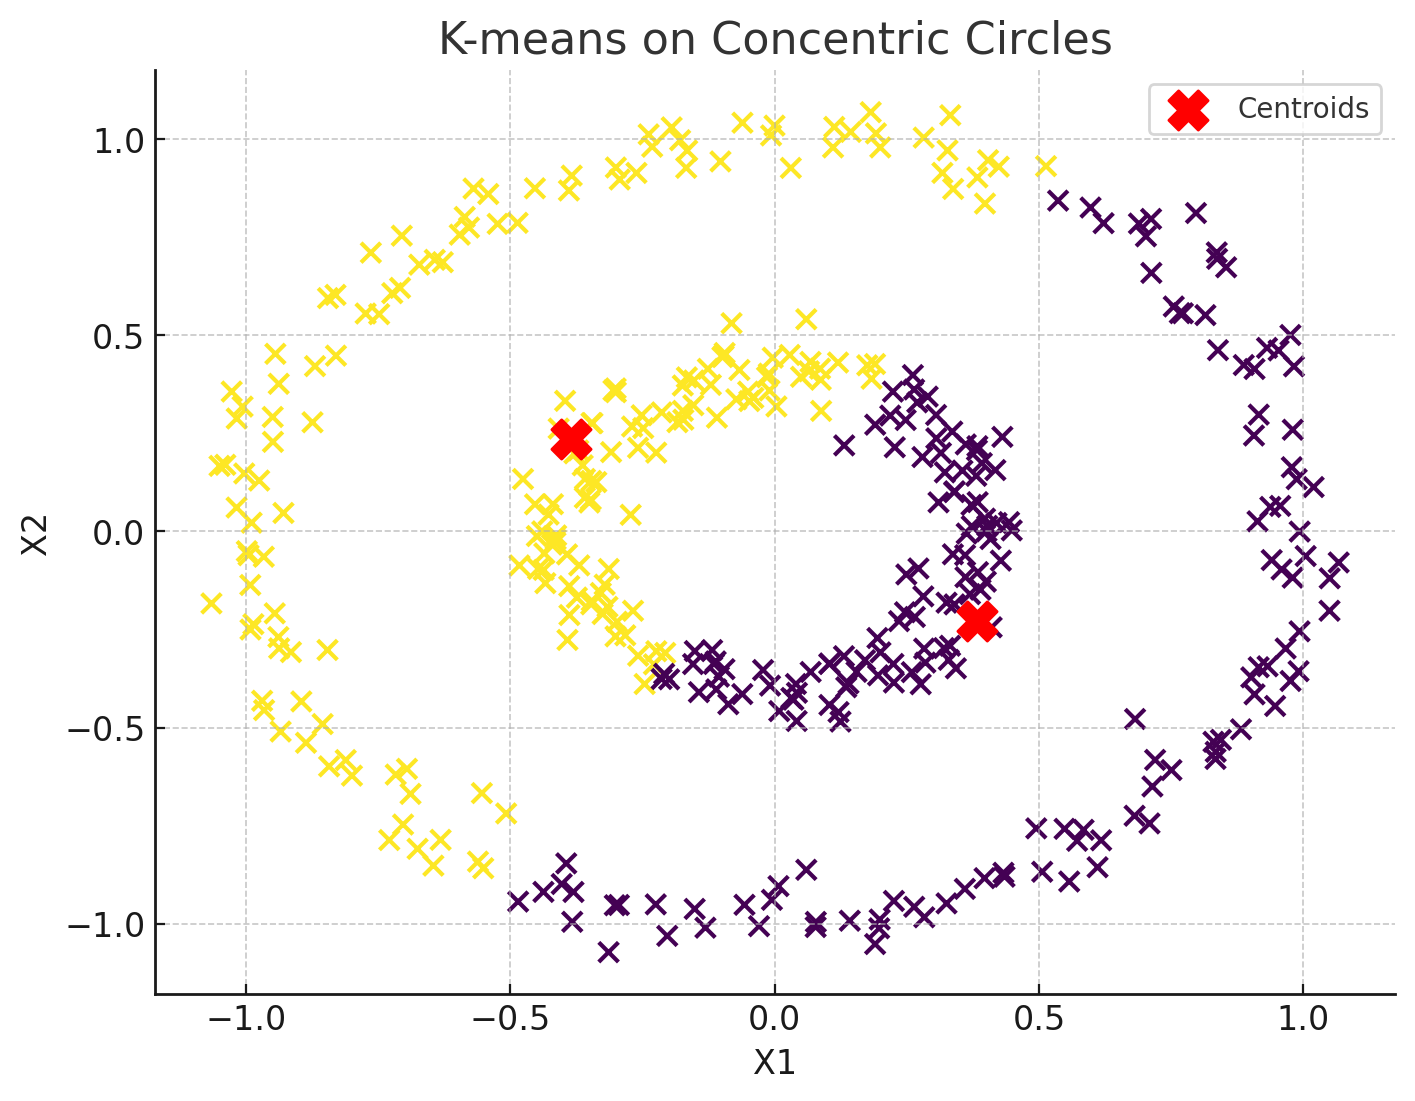
\includegraphics[scale=0.35]{pic/figs/kmeans_anti.png}
        \caption{example when k-means wont work, plot code generated by ChatGPT}
    \end{figure}

    \end{itemize}
\end{frame}


\section{Clustering}

\begin{frame}{Clustering}
    \begin{minipage}{0.95\textwidth}
        \begin{itemize}
        \item Assume we have a set of unlabeled data points $ \{ \mathbf{x}^{(i)} \}_{i=1}^N$.
        \item We intend to organize data into \textbf{groups }of \textbf{similar }objects.
        \begin{itemize}
            \item group and similar should be with respect to our need.
            \item For example all data points having most similar number of buys in a market.
        \end{itemize}
        \item A cluster is a collection of data items which are “similar” between them, and “dissimilar” to data items in other clusters.
        \item Clustering could also help to compress and reduce data. (???)
    \end{itemize}
    \end{minipage}%
    % \begin{minipage}{0.45\textwidth}
    %     \begin{itemize}
    %     \item Assume we have a set of unlabeled data points $ \{ \mathbf{x}^{(i)} \}_{i=1}^N$.
    %     \item We intend to find \textbf{groups of similar objects} with respect to our need.
    % \end{itemize}
    % \end{minipage}
\end{frame}

\begin{frame}{Clustering (cont.)}
    \begin{minipage}{0.55\textwidth}
        From another point of view, clusters are regions of high density that are separated from one another with regions of low density.
    % here we should talk what is good cluster ? should we even try to cluster based on density function ? should we focus of pure samples ? showcase the problem in which clustering could be both circle and a line extending of pmf (or pdf)
    \end{minipage}%
    \begin{minipage}{0.4\textwidth}
        \begin{figure}
            \centering
            \includegraphics[scale=0.5]{pic/clusteriong_pov.png}
        \end{figure}
    \end{minipage}
    \begin{tikzpicture}[remember picture,overlay]
        \node[anchor=south west, xshift=0.1cm, yshift=0.22cm] at (current page.south west) {
            \scriptsize Figure adapted from slides of Dr. Soleymani, Machine Learning course, Sharif University of technology.
        };
    \end{tikzpicture}
\end{frame}

\begin{frame}{Historic application of clustering}
\begin{itemize}
    \item John Snow, a London physician, plotted the location of cholera deaths on a map during an outbreak in the 1850s.
    \item The locations indicated that cases were clustered around certain intersections where there were polluted wells -- thus exposing both the problem and the solution.
\end{itemize}
    

\end{frame}

\begin{frame}{Modern applications of clustering}
\begin{itemize}
    \item Clustering is the origin of many unsupervised learning applications.
    \item Customer Segmentation (Marketing)
    \item Image Segmentation and Object Detection (Computer Vision)
    \item Anomaly Detection (Cybersecurity, Finance)
    \item Genomics and Bioinformatics
    \item Social Network Analysis and Community Detection
    \item Vector Quantization
    \item \dots
\end{itemize}
    

\end{frame}


\begin{frame}{Analysing the task}
\begin{itemize}
    \item first lets define a way to measure and show similarity. Two general ways would be:
    \begin{itemize}
        \item a similarity function $s(x_i,x_j)$ that is larger when $x_i$ and $x_j$ are more similar
        \item a dissimilarity or distance function $d(x_i,x_j)$ that is smaller the more simialr to points are.

    \end{itemize}
\item  a criterion to evaluate (and use to determine) a clustering. notion of "good" and "bad" clustering.
\item Algorithm to use the above and compute clustering.

            \item Extra Note: Most algorithms require a distance function to be a \textbf{proper metric} and the similarity measure to create a \textbf{PSD matrix} for all pairs of a finite number of data points.
\end{itemize}

    
\end{frame}


% \begin{frame}{Similarity measure and Distance measure}
    % \begin{minipage}{0.6\textwidth}
        % \begin{itemize}
        %     \item Similarity measures are used to distinguish between similar and non-similar data points.
        %     \item We usually define similarity of two data point as \textbf{inverse of distance} between them.
        %     \item Using this definition, {hard clustering aims to put data points with less distance in same cluster.}
        % \end{itemize}
    % \end{minipage}%
    % \begin{minipage}{0.35}
    %     \begin{figure}
    %         \centering
    %         \includegraphics[scale=0.4]{pic/Distance-based-clustering-approach.png}
    %     \end{figure}
    % \end{minipage}
% \end{frame}

\begin{frame}{Common similarity and distance measures}
    \begin{itemize}
        \item Assume \( p \) and \( q \) are two data points from $ \mathbb{R}^D$. most common similarity and distance measures in the problem of clustering are as follows:
        \begin{itemize}
            \item \textbf{Euclidean distance:} Most common measure of distance between two vectors:

            \[
            d(p,q)=\sqrt{{\sum_{i=1}^{D}{(p_i-q_i)^2}}}
            \]
            it is translation invariant.
            
            \item \textbf{Manhattan distance:} Most common measure of distance when dimensions are not equally important
            \[
            d(p,q)=\sqrt{\sum_{i=1}^{D} |p_i-q_i|}
            \]
            
            \item \textbf{Cosine similarity:} Most common measure of similarity when the magnitude of vectors does not change the similarity
            \[
            s( p,q)=\frac{p^T q}{||p|| \ . \ ||q||}
            \]

        \end{itemize}
    \end{itemize}
\end{frame}

\begin{frame}{Hard clustering vs Soft clustering}
    \begin{minipage}{0.55\textwidth}
        \begin{itemize}
        \item \textbf{Hard Clustering:} Each data point belongs to exactly one cluster
        \begin{itemize}
            \item more common and easier to do
        \end{itemize}
        \item \textbf{Soft Clustering}
    \end{itemize}
    \end{minipage}%
    \begin{minipage}{0.40\textwidth}
        \begin{figure}
            \centering
            \includegraphics[scale=0.5]{pic/hard_clustering.png}
        \end{figure}
    \end{minipage}
    \begin{tikzpicture}[remember picture,overlay]
        \node[anchor=south west, xshift=0.1cm, yshift=0.22cm] at (current page.south west) {
            \scriptsize Figure adapted from Machine Learning and Pattern Recognition, Bishop
        };
    \end{tikzpicture}  
\end{frame}

\begin{frame}{Hard clustering vs Soft clustering (cont.)}
    \begin{minipage}{0.55\textwidth}
        \begin{itemize}
        \item \textbf{Hard Clustering}
        \item \textbf{Soft Clustering:} Each data point can belong to multiple clusters.
        \begin{itemize}
            \item data point belongs to each cluster with a probability
        \end{itemize}
        \item \textbf{From now on, we will focus on problem of hard clustering}
    \end{itemize}
    \end{minipage}%
    \begin{minipage}{0.40\textwidth}
        \begin{figure}
            \centering
            \includegraphics[scale=0.5]{pic/soft_clustering.png}
        \end{figure}
    \end{minipage}
    \begin{tikzpicture}[remember picture,overlay]
        \node[anchor=south west, xshift=0.1cm, yshift=0.22cm] at (current page.south west) {
            \scriptsize Figure adapted from Machine Learning and Pattern Recognition, Bishop
        };
    \end{tikzpicture}  
\end{frame}

\begin{frame}{Cluster Evaluation}
    \begin{itemize}
        \item Intra-cluster cohesion (compactness)
        \begin{itemize}
            \item Cohesion measures how near the data points in a cluster are to the cluster centroid.
            \item Sum of squared error (SSE) is a commonly used measure.
        \end{itemize}
        \item Inter-cluster separation (isolation):
        \begin{itemize}
            \item Separation means that different cluster centroids should be far away from one another.
            \item Sum of squared error (SSE) is a commonly used measure.
        \end{itemize}
    \end{itemize}
\end{frame}

\begin{frame}{Clustering Algorithms}
\begin{itemize}
    \item The Traditional algorithms for clustering are usually categorized as: 
    \begin{itemize}
        \item \textbf{ Hierarchical} algorithms find successive clusters using previously established clusters. These algorithms can be either agglomerative ("bottom-up") or divisive ("top-down"):
\begin{itemize}
\item \textit{ Agglomerative } algorithms begin with each element as a separate cluster and merge them into successively larger clusters;
    \item \textit{ Divisive } algorithms begin with the whole set and proceed to divide it into successively smaller clusters.
\end{itemize}

\item \textbf{ Partitional } algorithms typically determine all clusters at once, but can also be used as divisive algorithms in the hierarchical clustering.

\item \textbf{ Bayesian} algorithms try to generate a posteriori distribution over the collection of all partitions of the data.

    \end{itemize}
\end{itemize}
\end{frame}


\begin{frame}{Clustering Algorithms (cont.)}
\begin{itemize}
    \item But modern approaches leverage advances in deep learning, self-supervised learning, and representation learning.
    \item As it is a common idea in ML, these methods transform data vectors, so the traditional clustering concepts can be applied.
    \item For example, with the same "curse of dimensionality" we had in supervised learning, for high dimensional vectors, using raw distance metrics will lose most of its functionality. So a Neural Network learns to transform data into a low dimensional space where our distance measure is more effective.
    \item Or when the data clusters are not centeric, they can be transformed into a space where the clusters are separated with respect to distance and in a centeric manner.

\end{itemize}
\end{frame}

\section{Conclusion}

\begin{frame}{Unsupervised Learning Review}
    \begin{itemize}
        \item \textbf{Objective}: To find hidden structures or underlying distributions in the data.
        \item \textbf{Input}: A dataset \( X = \{x_1, x_2, ..., x_n\} \subseteq \mathbb{R}^d \), where the data points \( x_i \in \mathbb{R}^d \) are unlabeled.
        \item \textbf{Goal}: Learn a mapping \( f: \mathbb{R}^d \to \mathbb{R}^m \) to describe underlying structure, in a way that is useful for a downstream task.
        \item Common tasks: 
        \begin{itemize}
            \item Clustering: The mapping \( f(X) = Z \) where \( Z \in \{1, 2, \dots, K\} \) represents the cluster assignments.
        
        \item Dimensionality Reduction: The mapping \( f(X) = Z \), where \( Z \in \mathbb{R}^k \) represents a lower-dimensional representation with \( k < d \).
        
        \item Density Estimation: Estimate the probability distribution \( P(X) \).
        \item Anomaly detection
        \item Generative modeling
        \end{itemize}
    \end{itemize}
\end{frame}

\begin{frame}{References}
    \begin{itemize}
        \item \cite{M2006-mk}
        \item \cite{MITNeuroscienceLecture2014}
        \item \cite{SontagMLLecture2012}
        \item \cite{soleymaniMLCourse}
        
    \end{itemize}
\end{frame}

\begin{frame}{Contributions}
\begin{itemize}
\item \textbf{This slide has been prepared thanks to:}
\begin{itemize}
    % \setlength{\itemsep}{10pt} % Adjust the value to control the spacing
    % \item \href{https://github.com/Mahan-Bayhaghi}{Mahan Bayhaghi}
\end{itemize}
\end{itemize}

\end{frame}

\begin{frame}[allowframebreaks]
    \bibliography{ref}
    \bibliographystyle{ieeetr}
    \nocite{*}
\end{frame}

\end{document}